\documentclass[report]{jsbook}
\usepackage[dvipdfmx]{graphicx}
\usepackage[dvipdfmx]{color}
\usepackage{booktabs}
\usepackage{latexsym}
\usepackage{okumacro}
\usepackage{fancybox,ascmac}
\usepackage{sty/algorithm}
\usepackage{sty/algorithmic}
\usepackage{colortbl}
\usepackage{multirow}
\usepackage{listings}
\usepackage{sty/jlisting}
\usepackage{url}
\usepackage{amsmath}
\usepackage{amsfonts}
\usepackage[noreplace]{otf}
\lstset{
	language={Java},
	basicstyle={\small},
	breaklines={true},
	frame=tRBl,
	framesep=5pt,
}

\newcommand\figref[1]{図\ref{#1}}
\newcommand\tabref[1]{表\ref{#1}}
\newcommand\equref[1]{式\ref{#1}}

\setcounter{tocdepth}{2}

\begin{document}
\pagestyle{empty}

\begin{center}

\vspace{5cm}

\textbf{\Large 卒業論文~2020年度(令和2年度)}

\vspace{2cm}

\textbf{\LARGE Depth2Jam:ドライブレコーダーを用いた渋滞推定システム}

\vspace{3cm}

\textbf{\underline{\large 指導教員}}\\
\textbf{慶應義塾大学環境情報学部}

% \textbf{\Large 徳田~~英幸}\\
\textbf{\Large 村井~~純}\\
\textbf{\Large 楠本~~博之}\\
\textbf{\Large 中村~~修}\\
\textbf{\Large 高汐~~一紀}\\
%\textbf{\Large 重近~~範行}\\
%\textbf{\Large 湧川~~隆次}\\
\textbf{\Large Rodney D. Van Meter III}\\
\textbf{\Large 植原~~啓介}\\
\textbf{\Large 三次~~仁}\\
\textbf{\Large 中澤~~仁}\\
\textbf{\Large 武田~~圭史}\\
%\textbf{\Large 加藤~~貴昭}\\

\vspace{6cm}

\textbf{\LARGE 慶應義塾大学 環境情報学部}

\vspace{.5em}

\textbf{\LARGE 李 広耀}

\vspace{.3em}

\textbf{\it koyo@ht.sfc.keio.ac.jp}

\newpage

\end{center}

\pagestyle{plain}

\frontmatter
\begin{center}
\textbf{\Large 卒業論文要旨 2020年度(令和2年度)}

\vspace{6.18mm}

\textbf{\Large Depth2Jam:ドライブレコーダーを用いた渋滞推定システム}
\end{center}

\vspace{10mm}

\begin{flushleft}
\textbf{論文要旨}\\
\end{flushleft}
日本において渋滞情報は主に道路に設置されているセンサーや監視カメラの映像から,逐次VICSなどの交通情報管理センターへ送られ,そこから自動車のナビゲーションシステム等に送信している.
しかし,現状渋滞情報を取得できるのは高速道路や国道などの一部の道路に限られており,そうでない道路では渋滞情報を収集できない.
また,ドライブレコーダーは近年の性能向上や危険運転や煽り運転の表面化の結果搭載率が高まっている.
しかし,搭載されたドライブレコーダーの映像を見るなどの活用をされるケースは少ない.
ドライブレコーダーは映像デバイスであるため物体検知や画像認識を行うことでさまざまなデーターを収集することが可能である.
本研究の目的は限られている渋滞情報が収集できるエリアを減らし,ドライブレコーダーの新しい活用方法を提案することである.
目的に対するアプローチとして,ドライブレコーダーの映像から渋滞推定を行うシステムDepth2Jamを提案する.
本研究ではDepth2Jamを実装し,渋滞推定精度について実験評価を行った.
また,Depth2Jamの精度について精度向上のための改善点と今後の展望について示した.

\begin{flushleft}
\textbf{キーワード}\\
\textbf{ドライブレコーダー,渋滞,深層学習,画像処理}

\end{flushleft}

\begin{flushright}
\textbf{慶應義塾大学 環境情報学部}\\
\textbf{李 広耀}
\end{flushright}
\newpage



\setlength{\baselineskip}{13pt}
\begin{center}
\textbf{\large Abstract of Bachelor's Thesis Academic Year 2020}

\vspace{6mm}

\textbf{\large Depth2Jam : Congestion Estimation System Using a Drive Recorder}

\end{center}

\vspace{10mm}


\begin{flushleft}
\textbf{Abstract}\\
\end{flushleft}
In Japan, traffic jam information is mainly obtained from sensors and monitoring cameras installed on roads, and sent to traffic information management centers such as VICS, which in turn send the information to car navigation systems.
However, traffic jam information can currently be obtained only on some roads, such as expressways and national ways, and cannot be collected on other roads.
In addition, the installation rate of drive recorders has been increasing as a result of recent improvements in performance and the surfacing of dangerous and incendiary driving.
However, there are few cases in which the videos from the installed drive recorders are used for viewing.
Since the drive recorder is a video device, it can collect various data by detecting objects and recognizing images.
The purpose of this research is to propose a new way to use the drive recorder and reducing the area where traffic jam information can be collected, which is limited.
As an approach to the purpose, we propose Depth2Jam, a system to estimate traffic jam from the images of drive recorders.
In this study, we implemented Depth2Jam and conducted an experimental evaluation of the accuracy of traffic jam estimation.
In addition, we show the improvement of the accuracy of Depth2Jam and its future prospects.

\begin{flushleft}
\textbf{Keywords}\\
\textbf{Drive Recorder,Traffic Jam, Deep Learning, Image Processing}
\end{flushleft}

\begin{flushright}
\textbf{Keio University Faculty of Environment and Infomation Studies.}\\
\textbf{Koyo Ri}\\
\end{flushright}


\setlength{\baselineskip}{16pt}
\tableofcontents
\listoffigures
\listoftables

\mainmatter
\chapter{はじめに}
本章では,はじめに本研究における背景とその目的等について述べる
\newpage
\section{背景}
% 背景と問題----------
日本はアメリカや中国などの道路と比較して国土が狭く、人口密度が高い。
それに伴って車道が狭く、渋滞が起こりやすくなっており、日々テレビやラジオのニュースで渋滞情報が報道されている。
渋滞の問題として、交通が滞ることによる物資や人員の運送の遅れだけでなく、ドライバーへの肉体的、精神的悪影響が挙げられる。
そのような背景のもと、ドライバーには渋滞情報をいち早く取得し、可能な限り渋滞を避けた運転をすることが求められている。

% 渋滞を減らすことを目指すのではなく、渋滞を推定することのメリットについて語るべきかもしれない。-----
日本では、渋滞情報は、VICS等の企業が道路に設置されているセンサーや車道付近に置かれているカメラの映像、および自動車に搭載されているセンサーやGPSの情報などをもとに算出されている。
また、日本におけるカーナビゲーションシステムはVICS等の渋滞情報を元に到着予想時刻などを割り出している。
VICSでは車両感知器(Vehicle Detectors)と光学式車両感知器の2つが主に使われ、それぞれ通過車両台数や渋滞情報を自動的に感知し交通管制センターへ送信する役割と、通過車両を感知するとともに車載装置との双方向の通信を行う役割を持っている。
加えて、渋滞情報はGoogle社が提供しているGoogle Mapにも提供されており、Web上でリアルタイムのデーターを閲覧することが可能である。
しかし、VICS等が管理している渋滞情報は、国道や高速道路といった日常的に交通量が多い道路には設置されているが、そうではない細い道や一方通行といった道では渋滞情報がない。

% 日本以外の交通情報について
日本以外の渋滞情報について、平成13年の警視庁によるトラフィック・インフォメーション・コンソーシアムでは、イギリス、ドイツ、アメリカの交通情報ビジネスについて述べられている\cite{traffic_buisiness}.
まずイギリスの交通情報ビジネスに関しては、Trafficmasterという企業が道路光津法の規定に基づき国からの免許を得て、さまざまな形で事業を展開している。
Trafficmasterの事業はイギリスだけにとどまらずドイツ、フランス、イタリア、オランダ、ベルギー等に及んでいる。
Trafficmasterは道路上に情報収集装置を設置し、赤外線センサーやカメラによって車両情報を読み取っている。
道路に情報収集装置を設置する点では日本における交通情報の取得と共通点がある。
次にドイツの交通情報ビジネスに関して、ドイツは高速道路網が発達しており、ダイムラー・クライスラーの子会社とドイツ・テレコムの共同出資によって設立されたTegaronや、イギリスのボーダフォングループに属するVodafone Tele Commerceによって交通情報ビジネスが行われている。
また、この両社が共同出資したDDGという企業は全国の高速道路に自ら設置した情報収集装置のほか、協力企業等の車両、警察や道路管理者等からの情報を統合し、上記の2社に情報提供を行なっている。
そしてアメリカでは、複数の民間事業者が道路交通情報ビジネスを行なっており、特にSmart Route Systemsという企業は全米21の大都市圏で事業を展開している。
日本を含めて、これら3カ国の道路交通情報の取得に関して共通しているのはどれも道路に情報収集装置を設置しているという点である。

\newpage

\section{ドライブレコーダーについて}
近年、煽り運転等のマナーの悪い運転が報道されるようになり、伴って各自動車へのドライブレコーダー搭載数が年々上昇している。
ドライブレコーダーは走行中の記録を撮ることにより事故の時の証拠を残すことができると同時に、事故等の証拠にもなり、警視庁も交通安全の面で、ウェブサイトにおいて取り付けを推奨している。
元々、煽り運転等の危険運転はドライブレコーダーが登場する前から発生していたが、近年社会問題として取り上げられているのはドライブレコーダーやスマートフォンなど、映像技術の向上により人々が気軽に高画質な映像を録画、記録することが可能になったからだと考えられる。
加えて近年のSNSの普及により、一般の人でも容易に事故の動画を発信したりと、注意喚起を行うことが可能になった。
結果、煽り運転のような危険運転が容易に可視化され、ドライブレコーダーや、スマートフォンで撮影した映像がニュースでも取り上げられるようになった。

% ドライブレコーダーの使用頻度の話を軽く ------------------
一般的なドライブレコーダーは事故の記録等で使われている。
しかし現状、ドライブレコーダーの搭載が増加しているにもかかわらず、そのほとんどの用途が事故等の、もしものための貯蔵となっている。
国土交通省の統計によると、ドライブレコーダーを取り付けた人のうち、実際にレコーダーの映像を見直すといった活用をしているのは2割ほどという結果が出ている\cite{ministryofland}。
ドライブレコーダーの映像からは先行車や道路の状態、歩行者など、さまざまなデータを取得することが可能であることを考えると、現状のドライブレコーダーを単純な映像記録装置として扱うのでは不十分であり、さまざまな機能をつけることで、より効果的、効率的に扱えるようになると言える。

\section{目的}
%この研究の目指すところについて述べる----------軽く
本研究の目指すところは、ドライブレコーダーから入力された画像および動画から、走行している場所が渋滞しているか否かを判断することにある。
ドライブレコーダーを使用して渋滞を推定することで、VICSやGoogle Map、そしてGPSの情報だけではでは見ることができない道路の渋滞の現場を可視化することが可能である。
VICSなどの道路に設置された情報収集装置と異なり、ドライブレコーダーはどのような自動車でも追加で取り付けることが可能であり、ドライブレコーダーで渋滞推定を行うことができれば、日本に限らず世界中の道路で渋滞推定を行うことができる汎用性がある。

加えて、本研究が目指すものは、渋滞の判断、評価のプロセスの次のフェーズとして、渋滞している場合、実際に渋滞している現場の画像及び映像をサーバーにアップロードすること、さらにその後のフェーズとして、ドライバー同士でそのような渋滞情報を共有することである。
交通の安全上、ドライバーは運転中にカーナビ等の電子機器を操作することは禁止されているため、システムが渋滞だと判断した場合、自動で渋滞データをアップロードする必要があり、また、渋滞データーはオープンな情報としてドライバーに共有される必要がある。
%以上の2つのフェーズを最終的に加えることで、このシステムの本来目指しているものは完成する。

\newpage

\section{渋滞の定義}
渋滞についての研究を行うためには、まず渋滞とはどのような状態か定義する必要がある。
普段我々がニュース等で情報を得ている渋滞情報として、日本道路交通情報センター(JATIC)は、高速道路では、時速40km以下で低速走行あるいは停止発進を繰り返す車列が、1km以上かつ15分以上継続した状態であるとし、一般道では、時速10km以下で低速走行している状態が渋滞であると定義している。
本研究では正確な速度をカメラ映像から割り出すことは不可能なため、それらの定義とは異なる独自の定義を使用する。
評価基準については5章の予備実験3の項で詳しく述べる。
%この研究で使っているGoogle Tensorflowが開発したStruct2depthシステムは画像及び動画のデーターを処理し、黄色と藍色の色の濃淡で距離を割り出している。
%カメラと位置が近ければ近いほど黄色い色が濃くなり、カメラから遠ざけば遠ざかるほど藍色の色が濃くなる。この研究では以上の状況を踏まえ、出力された画像及び映像から黄色い色の濃さの割合から先行車との車間距離を推定し、そこから速度を概算し、渋滞かどうか評価する。
%渋滞の定義においては、車道の自動車の数や交通量よりも走行速度の方に焦点が当たっている。

% 構成----------
\section{構成}
本論文の構成は以下の通りである。
2章で本稿で述べた問題について深く述べ、3章で問題にまつわる関連研究について述べる。
4章では本研究におけるアプローチとその設計と実装について述べる。
そして5章で本研究で実装したシステムに関して予備実験を行い、6章で本実験について述べる。
最後に7章で本実験に関して評価および考察を行い、8章で本研究のまとめについて述べる。
%\section{目的}
% この研究の目的を書く
ここでは本実験の目的について述べる。


%\chapter{渋滞とドライブレコーダー}
% Tanimu先輩"具体的に都市の画像を用いた想定している有効活用の方法について話す.軽く"
% 俺の研究の場合どんな問題について語ればいいんだろうねよくわからん
% 多分渋滞についての問題を書けばいいのかもしれない(適当)
ここでは本研究の主軸である渋滞とドライブレコーダーについて述べる.
\section{渋滞の原因}
まず,渋滞の原因について述べる.
大手自動車保険会社のチューリッヒ保険会社によると,渋滞は大きく交通集中渋滞,工事渋滞,事故渋滞の3種類に分けられる\cite{zurich}.
まず,工事渋滞と事故渋滞については,それぞれ工事や事故により道路区間の一部が通行できなくなり,渋滞が発生するというものである.
これら2つの渋滞は原因がはっきりしている.

しかし,交通集中渋滞に関しては一般的に原因があまり知れ渡っていない.
日本の高速道路の管理を行っているNEXCO東日本の調査によると,2018年に発生した渋滞のうち約73\%が交通集中事故だった\cite{NEXCOeast}.

また,交通集中渋滞が特に起きやすいとされている場所もあり,以下のようになっている.

\begin{itemize}
  \item 上り坂・サグ部
  \item 接続道路
  \item インターチェンジ
  \item トンネル
\end{itemize}

サグ部とは,下り坂から上り坂に変わる凹状の場所のことを指す.上り坂やサグ部では,無意識に速度が低下しがちである.
先行車の速度が低下すると,後続車が先行車の速度低下を確認し,次々とブレーキを踏む.
このようなメカニズムで渋滞がどんどん伸びてしまうのである.
NEXCO東日本の2018年の調査によると,高速道路にて発生した交通集中渋滞のうち66\%がこのような上り坂・サグ部で発生している\cite{NEXCOeast}.

接続道路とは,高速道路と一般道をつなぐ場所のことを指す.
高速道路の本線から一般道に出る地点に信号がある場合,青信号の間に車が一般道に出切らず,これが本線まで伸びて渋滞が発生することがある\cite{zurich}.

次にインターチェンジだが,接続道路と同じく,高速道路と一般道路との出入り口として設置されているインターチェンジの合流部は渋滞が多発するポイントである\cite{zurich}.
車両の流入に伴って,車線変更や速度を落とすといった自動車が多くなるため,後続車の速度も低下し渋滞となっている.

そして,トンネルに関して,トンネルの入り口は,急に暗くなり,圧迫感を感じることから,知らず知らずのうちにスピードを落として渋滞の原因になることがある\cite{zurich}.

\newpage

% --------------------------------------------------------------------------

\section{渋滞がもたらす影響}
渋滞中のドライバーには肉体的ストレスと精神的ストレスの両方がかかっている.
肉体的ストレスに関しては,運転中は長時間座ったままであり,狭い車内で体を伸ばすことができない,という問題が考えられる.
仮に遠出していて長時間渋滞に巻き込まれてしまうと同じ姿勢のまま運転する必要がありエコノミー症候群が発症する恐れが考えられる.
また,ドライバーの精神的ストレスに関して,東京農工大学大学院の佐藤氏\cite{alma99344256104031}は,渋滞中のドライバーの精神ストレスを以下のように述べている.

% -------------------------------------------------------------------

\begin{itemize}
  \item 目的地に早く着きたいのに自分の意に反して進めない \\
  \item 進もうとしているのに横入りにより邪魔される \\
  \item 退屈する \\
\end{itemize}

% ---------------------------------------------------------------------


また,自動車の交通渋滞はドライバーのみに影響を与えるのではない.
東京農工大学大学院の佐藤氏によると,渋滞中の交通事故の発生率は通常の時よりも8倍高い\cite{alma99344256104031}.
特に追突事故に関しては,通常の時よりも16倍高い事故発生率となる.

交通事故の原因の多くがヒューマンエラーによるものだと考えれば,渋滞情報を事前に取得し,渋滞を回避することは,ドライバーにとっても交通安全の面においても重要な課題なことがわかる.

\newpage

\section{渋滞検知}
% 渋滞情報はどのように作られるのか
% VICSの話
現在の渋滞は主要な道路にセンサーやカメラなどを取り付けてリアルタイムに渋滞情報を検知し管理している.
渋滞情報の取得には一般財団法人道路交通情報通信システムセンター(VICS)が関わっている.
VICSではVICSセンターが国土交通省,地方自治体および都道府県警察からの渋滞情報を集めて管理している.
集められた渋滞情報はFM多重放送,電波ビーコン,光ビーコンといった道路に設置された通信機でVICS対応カーナビゲーションシステムに送信し,渋滞情報や目的地までの到着予想時刻としてドライバーが受け取っている.
また,特に高速道路における渋滞情報の取得については,道路に2km間隔でトラフィックカウンターという計測器が埋め込まれており,通過する車の台数,大型車や小型車の区別,車の速度を計測している.
トラフィックカウンターだけではなく,高速道路においては交通管理隊が常に巡回しており,渋滞を見つけると無線で交通管制センターへ連絡し,ドライバーへフィードバックしている(参照:\figref{fig:vics_system}).

\begin{figure}[htbp]
  \begin{center}
   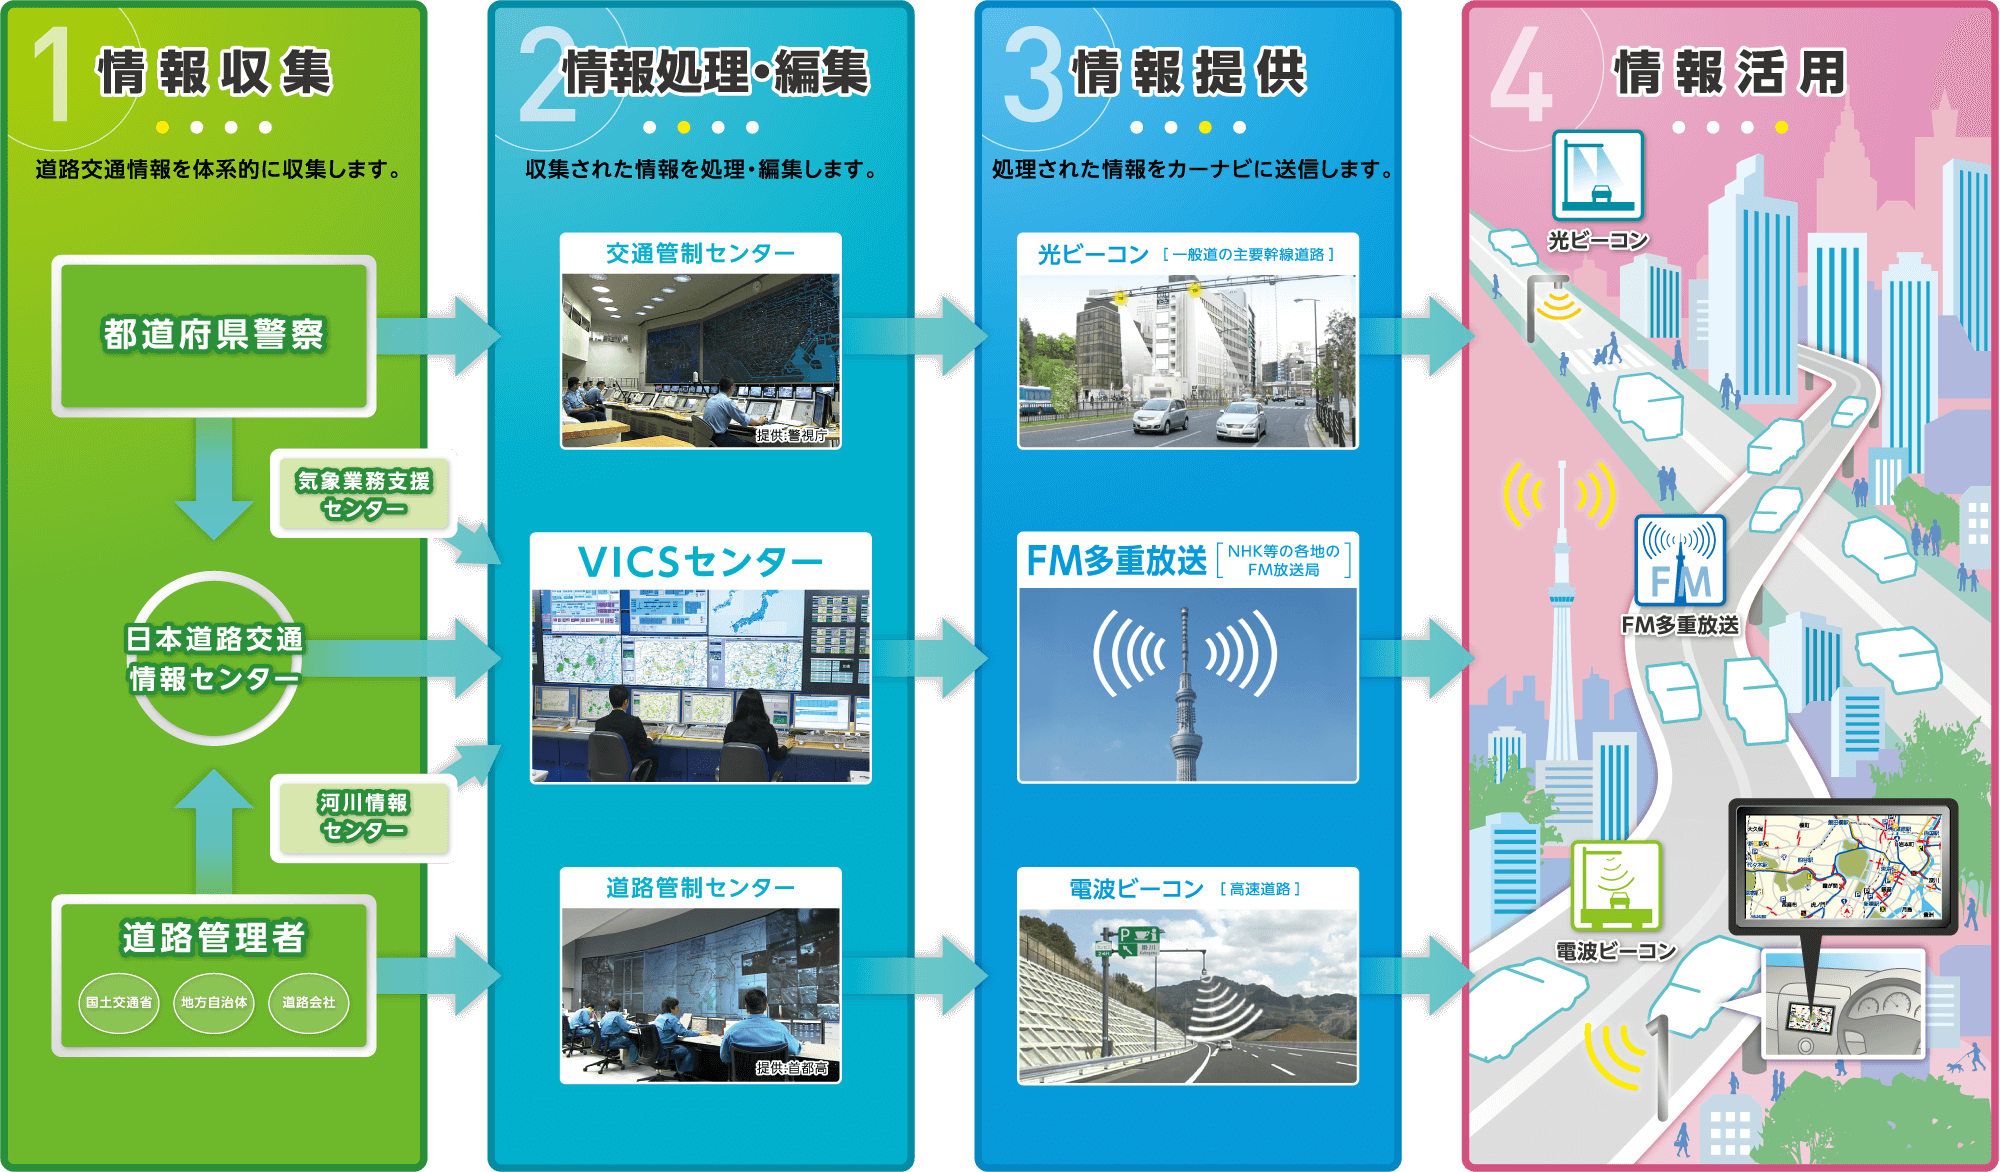
\includegraphics[width=11cm]{figs/vics.png}
  \end{center}
  \caption{VICSの仕組み(https://www.vics.or.jp/know/about/center.html)}
  \label{fig:vics_system}
\end{figure}

% それがどう不備なのか
しかし現状,渋滞情報は高速道路や国道といった主要な道路のみの情報しか得られておらず,それ以外の比較的小さい道路では渋滞情報を取得することができない問題がある.
例えば旅行シーズン中など,普段の走行量が少ない道路にて走行量が急に増えた際に,事前に渋滞情報を取得して迂回することが困難になる.
特に,1車線のような小さい道路が急な渋滞になるケースのことが多く,一度渋滞にはまってしまうと迂回ルートを取ろうとしても抜け出すことが難しくなる.

また,VICS非対応のカーナビゲーションが存在することも問題の一つである.
日本は世界的な自動車生産量を誇り,日本で走っている自動車はほとんどが国産車である.
しかし,2019年度の統計によると,日本市場における輸入車のシェアは6\%となっており,輸入車に載っている人口は一定数いることがわかる.
輸入車に乗っている人はVICS対応のカーナビゲーションを購入する必要がある.
また,日本で販売しているカーナビゲーションにもVICSに対応していない機種が存在する.

% プローブ情報を活用した例
\subsection{プローブ情報}
2020年よりVICSは渋滞ゼロ社会を目指すためにプローブ情報を利用したサービスの実証実験を行なっている(参照:\figref{fig:probe}).
プローブ情報とは,車一台一台の位置,速度,通過時刻等の等の走行軌跡データーを指す.
プローブ情報を活用することでこれまでトラフィックカウンターがなかった場所でも渋滞情報を取得することを目指し,実証実験を行なっている.

\begin{figure}[htbp]
  \begin{center}
   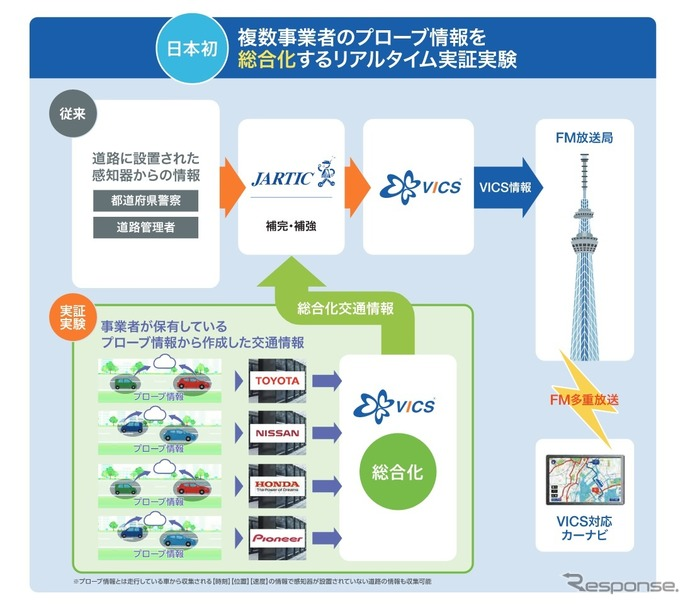
\includegraphics[width=11cm]{figs/probe.jpg}
  \end{center}
  \caption{実証実験中のプローブ情報を利用したシステム(https://response.jp/article/2020/03/05/332331.html)}
  \label{fig:probe}
\end{figure}

しかし,プローブ情報には車のセンサーを主に使っているため,ドライブレコーダーを使う等の情報はない.
センサーの情報のみを使って渋滞検知を行おうとすると,例えば低速運行しているのは渋滞に巻き込まれたからなのか,他の理由があるからなのか等の情報を得ることができない.
また,車が停止したのは渋滞のためなのか,停止信号のためなのか,あるいは駐車のためなのかといった情報もセンサーからのみでは得ることができない.
これらの情報を得るにあたって,ドライブレコーダーの使用は避けて通れないと考える.

% 渋滞に巻き込まれなくなることのメリットとか書いたほうがいいかな?
\newpage
\section{ドライブレコーダー}
% ドライブレコーダーの問題点
次に,ドライブレコーダーについて述べる.
% ドライブレコーダーの搭載率
2020年1月に国道交通省が出した統計\cite{ministryofland}によると,統計対象者のうちドライブレコーダーを実際に取り付けている割合は45.9\%という結果が出た.
つまり,統計の対象になったドライバーのうちおよそ半数がドライブレコーダーを搭載していることがわかる.
また,同統計において,ドライブレコーダーの使用目的のアンケートがあり,以下のようになっている.

% ----------------------------------------------------------------

\begin{table}[htbp]
  \centering
  \begin{scriptsize}
  \begin{tabular}{ccccccc}
  \toprule
ドライブレコーダーを & 安全運転の意識 & 自分の運転のクセなど & 交通事故の記録 & 煽り運転等  & 綺麗な風景など & その他 \\
なぜ導入するか(年代別) & を高める & を把握する & & 危険な運転への対策 & の記録 & \\ 
(複数回答可) & & & & & \\
  \midrule
全年代 & 45.5\% & 10.2\% & {\bf89.8\%} & {\bf71.7\%} & 7.7\% & 5.2\% \\
20代 & 50.0\% & 10,0\% & {\bf90.0\%} & {\bf63.3\%} & 16.7\% & 6.7\% \\
30代 & 38.9\% & 13.0\% & {\bf83.3\%} & {\bf74.1\%} & 7.4\% & 13.0\% \\
40代 & 46.1\% & 6.7\% & {\bf92.1\%} & {\bf76.4\%} & 11.2\% & 4.5\% \\
50代 & 47.4\% & 5.3\% & {\bf89.5\%} & {\bf59.2\%} & 5.3\% & 5.9\% \\
60代 & 42.1\% & 12.3\% & {\bf93.0\%} & {\bf78.9\%} & 3.5\% & 1.8\% \\
70代以上 & 57.9\% & 31.6\% & {\bf89.5\%} & {\bf84.2\%} & N/A & N/A \\
  \bottomrule
  \end{tabular}
  $\scriptstyle \mbox{出典:「自動車用の映像記録型ドライブレコーダー装置について」(国土交通省)}\atop \scriptstyle \mbox{(https://www.mlit.go.jp/monitor/R1-kadai01/24.pdf)}$
\end{scriptsize}
  \caption{ドライブレコーダー導入の目的(年代別)}
  \label{tab:recoder_static_age}
\end{table}

\begin{table}[htbp]
  \centering
  \begin{scriptsize}
  \begin{tabular}{ccccccc}
  \toprule
ドライブレコーダーを & 安全運転の意識 & 自分の運転のクセなど & 交通事故の記録 & 煽り運転等  & 綺麗な風景など & その他 \\
なぜ導入するか(地域別) & を高める & を把握する & & 危険な運転への対策 & の記録 & \\ 
(複数回答可) & & & & & \\
  \midrule
北海道 & 43.5\% & 17.4\% & {\bf91.3\%} & {\bf87.0\%} & 4.3\% & 4.3\% \\
東北 & 51.9\% & 11,1\% & {\bf85.2\%} & {\bf74.1\%} & 7.4\% & 3.7\% \\
関東 & 44.4\% & 12.7\% & {\bf82.5\%} & {\bf66.7\%} & 7.9\% & 7.9\% \\
北陸 & 63.0\% & 22.2\% & {\bf85.2\%} & {\bf74.1\%} & 7.4\% & 3.7\% \\
中部 & 36.4\% & 9.1\% & {\bf93.2\%} & {\bf77.3\%} & 9.1\% & 6.8\% \\
近畿 & 38.9\% & 1.9\% & {\bf94.4\%} & {\bf70.4\%} & 3.7\% & 3.7\% \\
中国 & 39.3\% & 7.1\% & {\bf89.3\%} & {\bf57.1\%} & 17.9\% & 7.1\% \\
四国 & 56.5\% & 17.4\% & {\bf91.3\%} & {\bf69.6\%} & N/A & 4.3\% \\
九州 & 50.0\% & 2.8\% & {\bf97.2\%} & {\bf75.0\%} & 11.1\% & 2.8\% \\
  \bottomrule
  \end{tabular}
  $\scriptstyle \mbox{出典:「自動車用の映像記録型ドライブレコーダー装置について」(国土交通省)}\atop \scriptstyle \mbox{(https://www.mlit.go.jp/monitor/R1-kadai01/24.pdf)}$
\end{scriptsize}
  \caption{ドライブレコーダー導入の目的(地域別)}
  \label{tab:recoder_static_block}
\end{table}

% -------------------------------------------------------

表から分かる通り,どの年代およびどの地域でも,ドライブレコーダーを取り付ける目的としては「交通事故の記録」が最も高く,次いで「煽り運転等危険な運転への対策」,「安全運転の意識」が高くなっている.
また,同統計ではドライブレコーダーの活用状況についての統計があり,\figref{fig:use_recoder}と\figref{fig:use_recorder2}に結果を示す.

また,ドライブレコーダーを実際にどのように活用したかについてのアンケート結果があり,\tabref{tab:howto_use_rec}に結果を示す.
以上のことからわかることは,統計に参加したドライバーのうち約半数がドライブレコーダーを取り付けて入るものの,実際にドライブレコーダーの映像を活用できているのは全体の2割ほどであるということである.

%----------------------------------

\begin{figure}[htbp]
  \begin{center}
   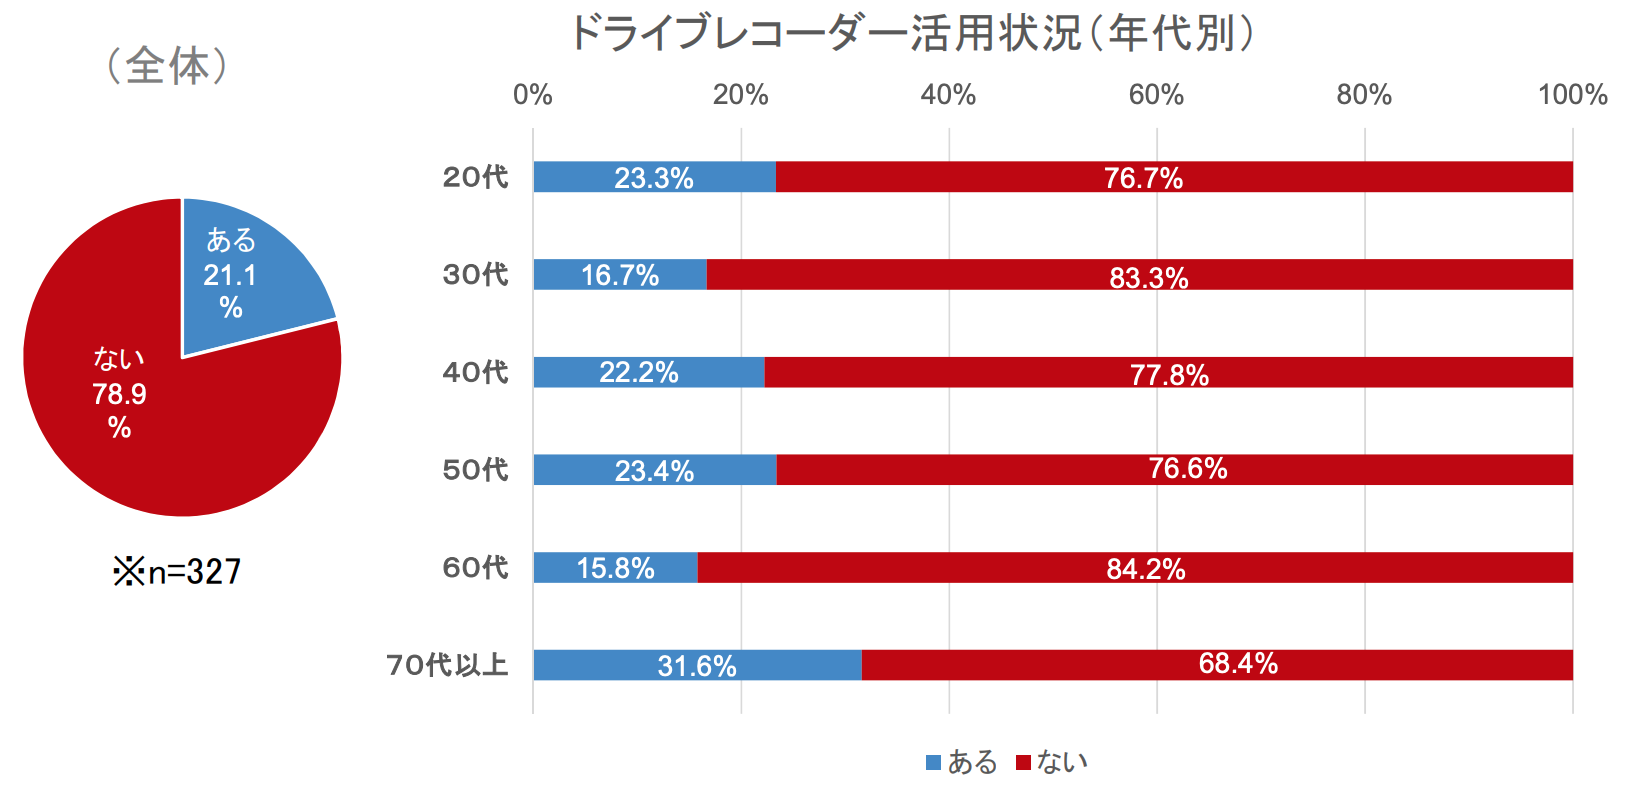
\includegraphics[width=12cm]{figs/use_driverecoder1.png}
   $\scriptstyle \mbox{出典:「自動車用の映像記録型ドライブレコーダー装置について」(国土交通省)}\atop \scriptstyle \mbox{(https://www.mlit.go.jp/monitor/R1-kadai01/24.pdf)}$
  \end{center}
  \caption{ドライブレコーダーの記録を活用したことがあるかについてのアンケート結果(年代別)\cite{ministryofland}}
  \label{fig:use_recorder}
\end{figure}

\begin{figure}[htbp]
  \begin{center}
   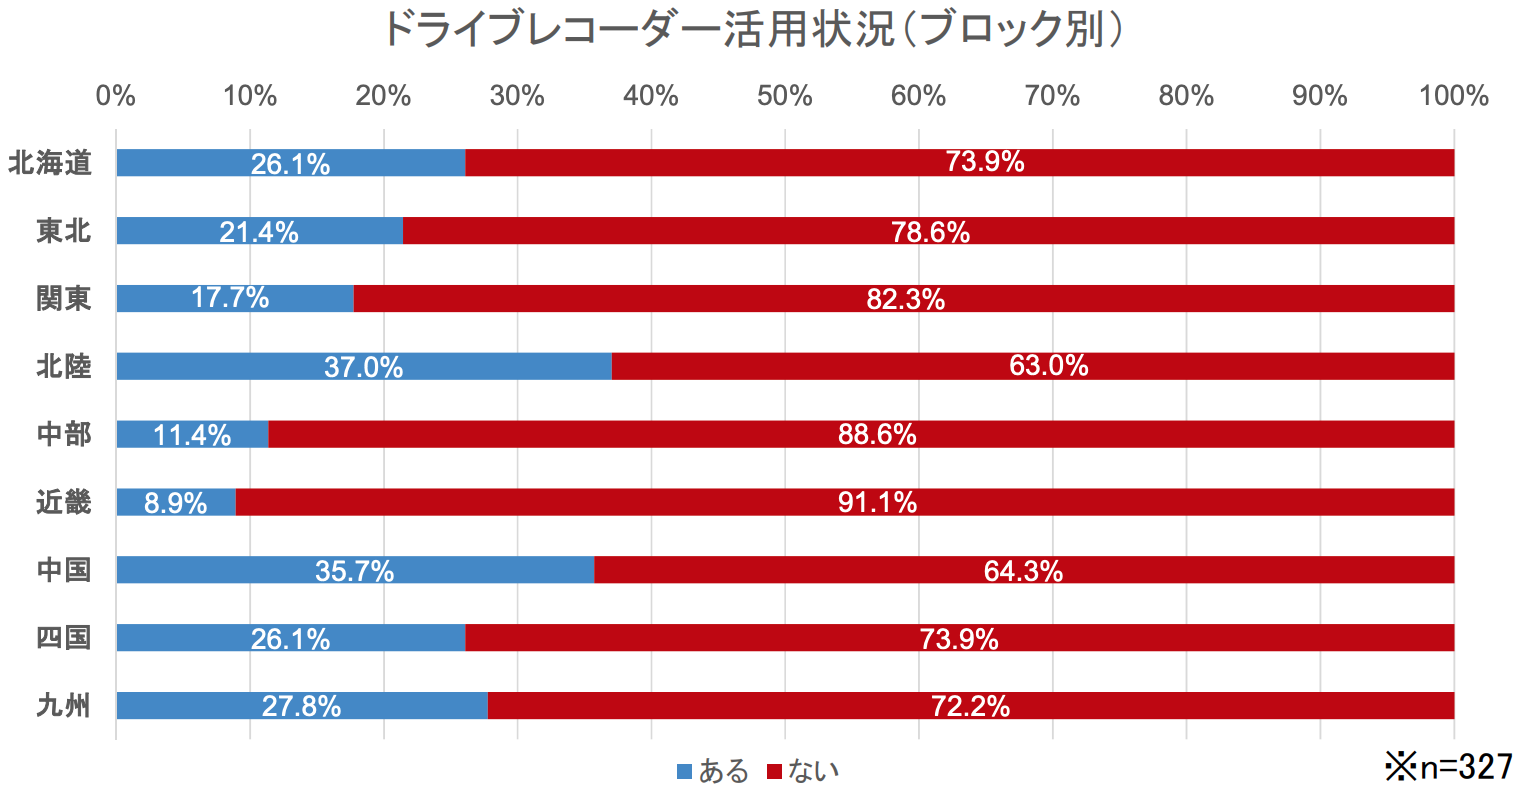
\includegraphics[width=12cm]{figs/use_driverecorder2.png}
   $\scriptstyle \mbox{出典:「自動車用の映像記録型ドライブレコーダー装置について」(国土交通省)}\atop \scriptstyle \mbox{(https://www.mlit.go.jp/monitor/R1-kadai01/24.pdf)}$
  \end{center}
  \caption{ドライブレコーダーの記録を活用したことがあるかについてのアンケート結果(ブロック別)\cite{ministryofland}}
  \label{fig:use_recorder2}
\end{figure}

\begin{table}[htbp]
  \centering
  \begin{scriptsize}
\begin{tabular}{cc}
  \toprule
状況 & ドライブレコーダーをどのように活用したか\\
  \midrule
交通事故の時 & 貰い事故の際に,自分の無過失が証明できた.\\
& 交通事故に遭遇した際に,第三者として記録を提出した. \\
\hline
安全運転のため& 悪質な運転や犯罪の動画をもとに警察へ通報した.\\
& 事故になりかけた状況を,後日再確認した.\\
& 家族でお互いの運転を検証している.\\
& 車内での安全運転啓発に画像を利用した. \\
& 運転中に相手車の運転を確認する. \\
& 危険運転などの動画をSNSに投稿した.\\
\hline
その他 & 豪雨災害や隕石の落下などたまたま映っていた画像を共有した.\\
& 旅先などの景色や遭遇した野生動物などを録画した.\\
\bottomrule
\end{tabular}
$\scriptstyle \mbox{出典:「自動車用の映像記録型ドライブレコーダー装置について」(国土交通省)}\atop \scriptstyle \mbox{(https://www.mlit.go.jp/monitor/R1-kadai01/24.pdf)}$
  \end{scriptsize}
  \caption{ドライブレコーダーの活用状況}
\label{tab:howto_use_rec}
\end{table}

% ---------------------------------------------------------------------

\newpage
\section{ドライブレコーダーを使うメリット}
2.2章で述べた通り,ドライブレコーダーを設置している人口は一定数いるものの,そのほとんどがドライブレコーダーを実際に活用していないことがわかる.
本研究ではドライブレコーダーからの車間距離を推定することで渋滞を推定することを目的としているが,この車間距離の推定をすることでいずれは煽り運転の推定や警告などドライバーにとって有益な情報提供ができる研究に繋げることが可能だと考えられる.
また,車間距離を推定することができれば,安全運転を評価することも可能になる.
世界の情勢として,自動運転への移行に舵がとられているが,日本では法整備の問題等で完全な自動運転への移行は未だに時間がかかると予想されている.
ドライブレコーダーの映像から得られる情報は,ドライバーの見ている景色とほぼ同じだとすると,ドライブレコーダーを使って渋滞だけでは無く,道路標識や信号等も検出することが可能である.
それらの検出をもとに,ドライバーがきちんと道路標識に従って,一時停止等していたか,十分な車間距離を守って走行できていたか,というようなドライバーが安全運転だったか否かを評価することができる.
これは他のセンサーやGPSのデーターだけを用いる手法では難しく,ドライブレコーダーを活用する利点であると言える.
さらに,先行車の動きをトラッキング,分析することで煽り運転の検出,警告することも可能である.


\section{まとめ}
本章では渋滞とドライブレコーダーの諸問題について述べた.
次章では本研究の関連研究について述べる.
\chapter{関連研究}
%ドライブレコーダーを用いた関連研究について
\section{ドライブレコーダーを用いた研究}
自動車にカメラ及びドライブレコーダーを取り付けて行なった研究として、まず道路のひび割れや塗装の剥がれといったものを検出する研究\cite{全邦釘2017ディープラーニングおよび}がある。
画像処理技術が向上したことで、道路における障害物やひび割れといったものの検出が可能となった。
しかし、道路のひび割れのような不動で固定的なものとは異なり、渋滞というものは時間と共に発生したり解消したり、また規模も大きくなったり小さくなったりと変化するものあり、変化するものに対しての画像認識の対応は困難なものだった。

ドライブレコーダーと機械学習を組み合わせたものとしては、Japan Taxi株式会社が既にタクシーに高性能なドライブレコーダーをつけて、走行中の道路の状況等をリアルタイムに収集し解析するというサービスを行なっている。
しかし、そこで行われているのは歩行者の検出や道路工事の検出などであり、発展して渋滞を推定すると言う旨の実現には至っていない。
各タクシーから集められた情報をもとに人間の手で渋滞かどうか判断しているので、本研究によってその人間の判断を自動化する、あるいは事前に渋滞かどうか疑わしい現場の映像に判断材料を絞ることができる点で、本研究には貢献できる点があると言える。

%車載カメラからの画像処理について書きたい
\section{ドライブレコーダー以外の車載カメラを用いた研究について}
ドライブレコーダー以外の車載カメラの研究について、三上ら\cite{三上量弘2020deepcounter}は、ゴミ収集車にカメラ取り付けるとこで、ゴミ収集車にどれほどのゴミ袋が収集されたかを調べる研究を行った。
ゴミ清掃車は、日々決まったルートを通り、決まった場所でゴミを収集している。
その収集されるゴミの量を数値として可視化することで住民の生活の変化を可視化する研究である。
自動車にカメラを取り付けて、映像情報からデーターを可視化するという目的の点で、可視化するデーターが異なるとはいえ、三上らの研究はこの研究と共通点がある。
また、三上らの研究には私の研究と同様のYOLOと呼ばれる物体検出システムが使用されており、その物体検出システムが検出したゴミ袋の量を計測していた。

以上を踏まえると、物体検出システムを使用することでデーターの可視化が可能であると言える。

\newpage

\section{渋滞推定の研究について}
ドライブレコーダー以外の方法でカメラから渋滞を測定する方法として、進藤ら\cite{進藤瞭2013車載カメラ画像を用いた対向車線の渋滞状況の把握手法}は、対向車の交通量を測定することで渋滞を推定する研究を行なった。
進藤らの方法は自動車2台を走行させ、その2台の横を通過した対向車の数から渋滞しているか否かを判断するものである。
しかし、進藤らの方法では測定するための自動車は常に道路の右側車線を走行しなければならないと同時に、対向車道がない道路では渋滞を推定することができないという問題がある。

\section{カメラを用いた距離推定の研究}
%センサー情報を含めた先行研究
車間距離を推定するフェーズに関して、動画から距離を推定する方法はいくつか存在する。
まず最も簡単かつ確実な方法は複眼カメラと三角関数を利用した方法である。
同じ対象を移したときに2つの視点からそれぞれのカメラから対象の距離を測定する方法である。
しかし、本研究の対象はドライブレコーダーであり、1つの自動車に2つのドライブレコーダーを搭載することは現実的ではなく、複眼のドライブレコーダーは一般的に搭載されていないためこの方法は利用できない。
そのため、この研究では単眼カメラの映像から車間距離を推定する必要がる。
単眼カメラから物体との距離を推定する研究としては、カメラ情報に加えて各種距離センサーの情報を利用することで実現する方法が一般的であった。

% Struct2depth
しかし、近年ではDeep Learning技術の向上により、各種センサーといった教師データーのない、純粋に画像のみでの距離推定プログラムが実現している。
Zhouら\cite{zhou2017unsupervised}はセンサー情報等の教師データのないカメラ映像から奥行きを推定するシステムを開発した。
Zhouらのシステムは、車載動画等の連続的な画像の集まりであるデータセットを元に映像における視界の変化を元に奥行きを推定するものであった。
Zhouらの研究以降、カメラ映像における奥行きの研究は、Zhouらの研究を元に性能向上がなされ、Yinら\cite{yin2018geonet}などによってアップデートがなされた。

中でも、Googleの研究チームのCasserらが行なった研究である"Struct2Depth"\cite{casser2019struct2depth}というシステムは上記の研究と比較して精度がより向上されている\figref{fig:depth_related}。
本研究ではStruct2Depthを利用し、車間距離を推定する。

\newpage

\begin{figure}[hp]
  \begin{center}
   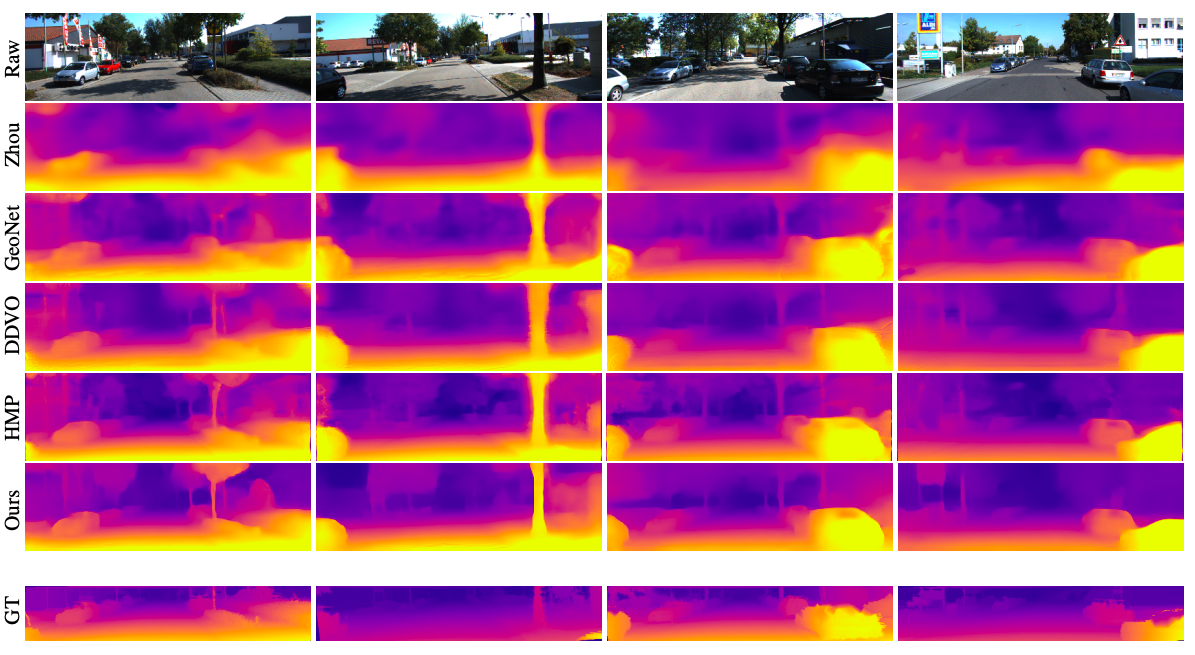
\includegraphics[width=\textwidth]{figs/struct2depth_related.png}
  \end{center}
  \caption{struct2depthと他の研究の比較\cite{casser2019struct2depth}}
  \label{fig:depth_related}
\end{figure}

\begin{figure}[hp]
  \begin{center}
   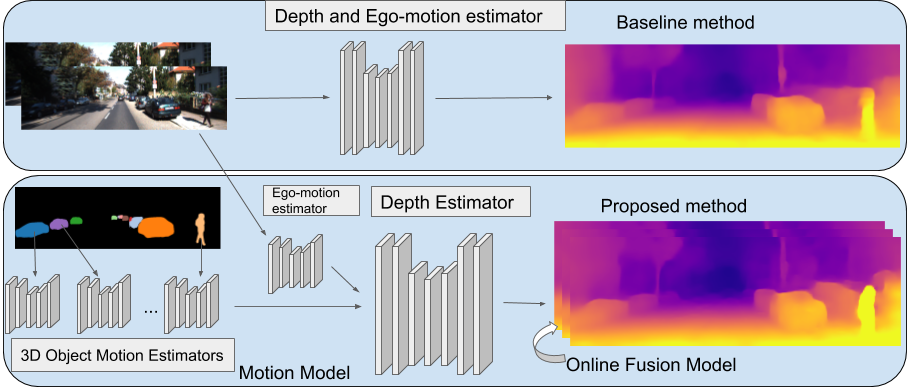
\includegraphics[width=\textwidth]{figs/aproach_depth.png}
  \end{center}
  \caption{struct2depthのアプローチ(https://sites.google.com/view/struct2depth)}
  \label{fig:approach_depth}
\end{figure}

\newpage
\section{物体検出システムについて}
%YOLOとかの話
物体検出を行うライブラリは様々あり、Fast R-CNNs\cite{ren2015faster}、Mask R-CNN\cite{he2017mask}、SSD\cite{liu2016ssd}といった手法が挙げられる。
それぞれCNNと呼ばれる畳み込みネットワークを利用し物体検出を行なっている点は同じだが、CNNの層や物体検出を行う際の手法がわずかながらに異なっている。
本研究では物体検出手法としてYOLO(You Only Look Once)\cite{yolov3}\figref{fig:yolo_system}\figref{fig:yolo_network}と呼ばれる物体検出手法を用いる。
YOLOは上記の3つの手法と比較して畳み込みネットワークやニューラルネットワークがシンプルな構造になっているにもかかわらず、高い検出率を誇っている。
また、構造が比較的シンプルなため演算処理にかかるスピードが速く、リアルタイムでの処理にも適している。
本研究では、YOLOがMicrosoft COCO datasetを機械学習したものを利用し、ドライブレコーダーに写っている自動車、トラック、バスを主に検出させ、距離推定及びその結果からシステムの評価を行う。


\begin{figure}[htbp]
  \begin{center}
    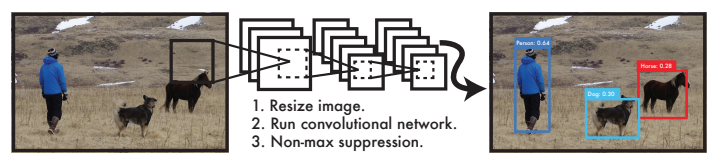
\includegraphics[width=\textwidth]{figs/Yolo_Detection_system.png}
    \caption{YOLOの物体検出システム\cite{yolov3}}
    \label{fig:yolo_system}
  \end{center}
\end{figure}

\begin{figure}[htbp]
  \begin{center}
    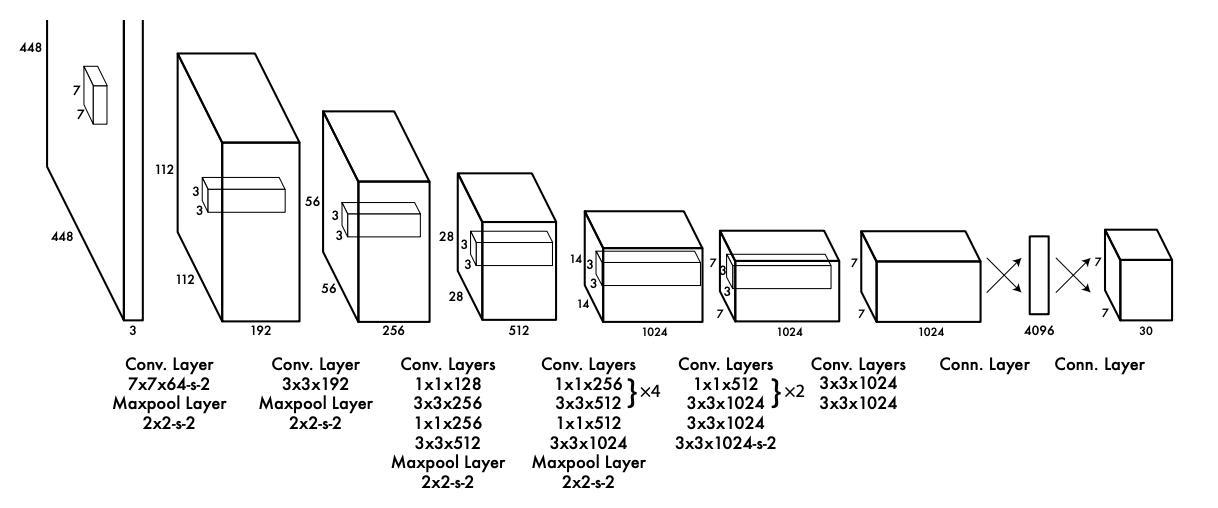
\includegraphics[width=\textwidth]{figs/yolo_architecture.png}
    \caption{YOLOのネットワーク構成図\cite{yolov3}}
    \label{fig:yolo_network}
  \end{center}
 \end{figure}

 \section{まとめ}
 本章では本研究における関連研究について述べた。
 次章では、問題に対する本研究のアプローチおよび本研究のシステムの設計と実装について述べる。
\chapter{アプローチ}
本研究ではドライブレコーダーの映像から自動車を検出,車間距離を推定し,渋滞しているか否かを判断するシステムを提案する.
本章では,自動車の検出と車間距離を推定する手法とそのネットワーク構造について述べる.

\newpage

\section{設計}
\subsection{研究手法}
本研究では,汎用性を重視するためにドライブレコーダーから得られる情報のみを利用する.
渋滞の定義の項でも述べたが,渋滞を推定するためには速度が重要だが,ドライブレコーダーと自動車の速度を同期させるためには専用の取り付け工事が必要であり,また車の種類や自動車メーカーによって内部構造は異なっている.
また,映像から速度を推定する方法も手法の一つとして考えられるが,映像から速度を出すためには相対距離の算出が必要であり,リアルタイムの情報が求められているこの研究では相対速度を計算する処理は処理時間を増やす原因を作ると同時に,映像から正確な速度情報を算出することは非常に困難である.
また,速度センサーを搭載して速度を求める方法も考えられ,加速度センサーの使用が考えられる。
しかし、現状加速度センサーが搭載されている市販のドライブレコーダーは存在しないため、状況が限られてしまい、汎用性が担保できない問題が発生する。
また、加速度センサーが搭載されているスマートフォンを自動車に取り付けて速度推定を行う方法も考えられる。
一般的に、速度は加速度を積分することでその時々の速度を推定することができるが、不良積分が多く発生してしまう恐れがあると同時に、物体検出、速度推定に加えてそのような加速度センサーデータから速度を計算すると機械が処理するものが多くなり、映像の処理におけるFPSが低下する恐れがある。
このFPSの低下はリアルタイムでの処理を目指すこの研究において重大な欠陥となってしまう。

さらに、GPSを用いて渋滞を推定する方法もあるが、ドライブレコーダー等の映像記録装置は実際に映像を取得できる利点があるのに対して、GPSは位置情報データーを取得するため、得られる情報に限りがある。
その上、GPSのみで渋滞情報を取得する方法は例えばGPSを搭載した電子機器を複数自動車に持ち込むと、実際には渋滞していないのにもかかわらず、渋滞していると出力してしまうような事例がある[出典]ため、実際に渋滞の現場を確認することができると言う点でドライブレコーダーを使う方法が最も汎用性が高い。
それに加えて、速度だけで判断してしまうと、例えば自動車が停止したとき、渋滞のために停止したのか、信号のために停止したのか、あるいは駐車したために停止したのか、判断することができない、という問題が発生してしまう。
近年では自動運転技術等の向上により、障害物に近づくとドライバーに警告するようなセンサーを搭載した高性能な自動車も存在するが、この研究ではより汎用性を重視するため、ドライブレコーダーの情報のみで渋滞の推定を行う。

%\section{物体検出を用いた方法}
%試行錯誤について書いてみよう
\newpage
\section{実装}
\subsection{ネットワークアーキテクチャ}
% システムの構成について書く
本研究はドライブレコーダーの映像から自動車を検出するフェーズと同じく映像から先行車との車間距離を推定するフェーズの2つのフェーズから構成されている。
設計の項でも述べた通り、ドライブレコーダーにおける渋滞推定手法は物体検出システムと深度推定システムを用いる。
本研究におけるネットワークアーキテクチャを\figref{figs:system_arch}に示す。
また、渋滞かどうか判断するまでのフローチャートを\figref{fig:system_flow}に示す。

\begin{figure}[htbp]
  \begin{center}
    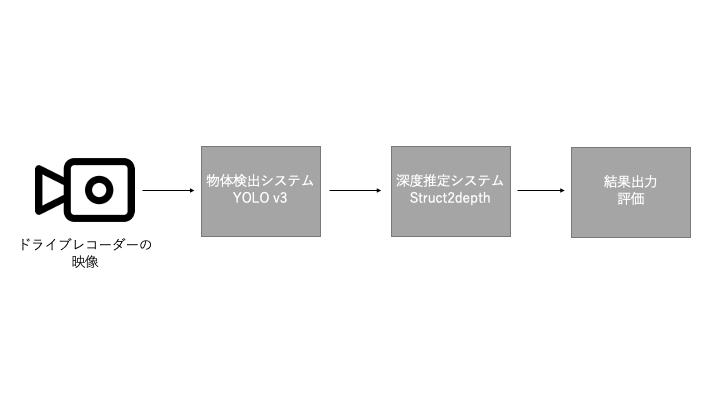
\includegraphics[width=12cm]{figs/system_buildver1.png}
    \caption{ネットワーク構成図}
    \label{fig:system_arch}
  \end{center}
\end{figure}


% 自動車の検出について---
\subsection{自動車検出}
まず、入力された動画から車を検出するフェーズでは、画像認識技術を利用して、車を検出している。
物体検出を行うライブラリは様々あり、Fast R-CNNs、Mask R-CNNs、SSDといった手法が挙げられる。
それぞれCNNと呼ばれる畳み込みネットワークを利用し物体検出を行なっている点は同じだが、そのCNNの層や物体検出を行う際の手法がわずかながらに異なっている。
本研究では物体検出手法としてYOLO(You Only Look Once)と呼ばれる物体検出手法を用いる。
このシステムは物体を検出するとその物体をBounding Box(BBOX)と呼ばれる四角形で囲むことでその物体の映像における位置を示すものである。
YOLOは上記の3つの手法と比較して畳み込みネットワークやニューラルネットワークがシンプルな構造になっているにもかかわらず、高い検出率を誇っている。
また、構造が比較的シンプルなため演算処理にかかるスピードが速く、リアルタイムでの処理にも適している。
本研究では、YOLOがMicrosoft COCO datasetを学習したものを利用する。

\subsection{距離推定}
本研究ではGoogle Tensorflowが開発したStruct2Depthシステムを利用する。
struct2depthは入力された映像から奥行きを推定し、カメラとの距離が近いほど明るい色に、遠いほど暗い色に色分けすることによって奥行きを可視化する。
本研究ではそのシステムを利用し、自動車が検出されたBBOXの場所と同期させることでその明るさから先行車との車間距離を推定する。

\subsection{処理軽減化}
\figref{fig:system_arch}の通り、本研究の実装する渋滞推定システムは、映像情報を物体検出ライブラリ(YOLOv3)を用いて自動車を検出した後、深度推定ライブラリ(YOLO v3)を用いて距離を推定するという順番である。
本研究におけるシステムの設計として、当初はドライブレコーダーの映像を深度推定ライブラリ、物体検出ライブラリと、処理する順番が逆であった。
しかし、処理にかかる時間と量を顧みて、先に物体検出ライブラリを用いて自動車を検出し、自動車が検出されたことが確認できた時のみ、深度推定ライブラリ用いて車間距離を推定するという方針にした。
この変更によって処理時間を軽減化するだけでなく、処理にかかる時間を短くすることに成功した。
(具体的な処理軽減率等についてはおいおい実験します)

\begin{figure}[htbp]
  \begin{center}
    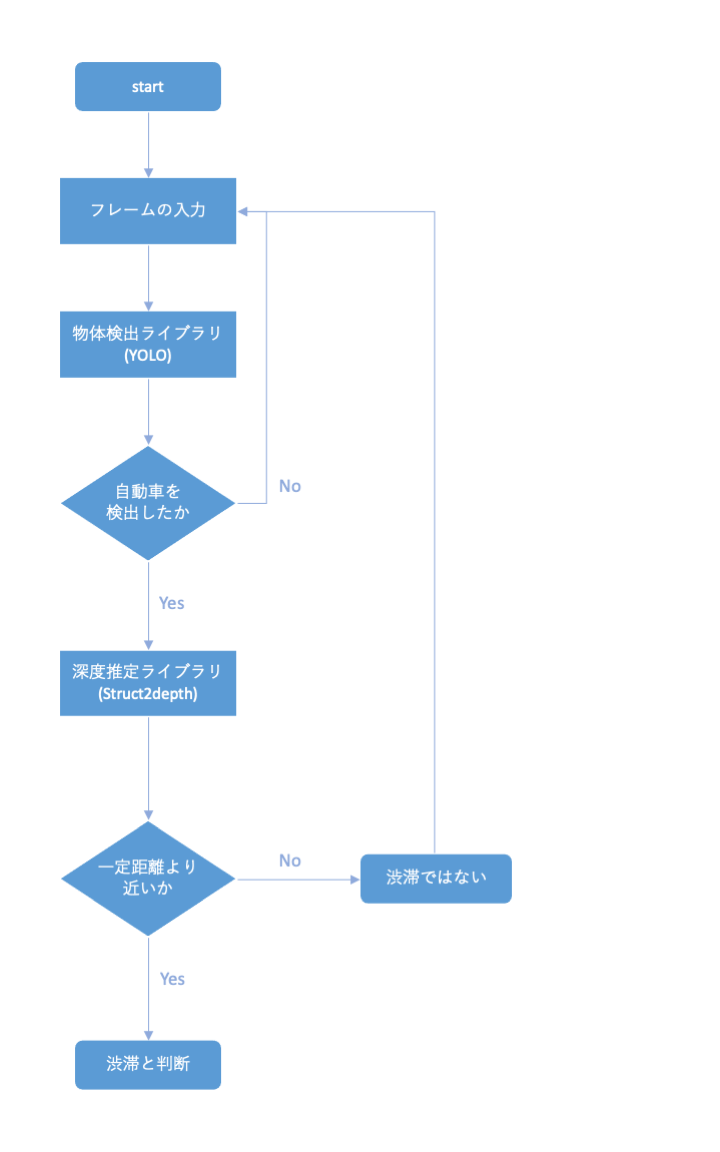
\includegraphics[width=10cm]{figs/gp2_flowchart.png}
    \caption{フローチャート}
    \label{fig:system_flow}
  \end{center}
\end{figure}

\section{渋滞の評価について}
ここでは渋滞の評価方法について述べる。
背景の項でも述べた通り、日本において渋滞の定義は自動車の運行スピードに依存しているが、本研究においては正確なスピードを取得するのは困難なため、先行車との車間距離を推定することで、その推定された距離を元に渋滞しているかどうかを判断する。

\section{まとめ}
本章では、本研究におけるアプローチとシステムの設計及び実装について述べた。
次章では本章で述べたシステムの実装に伴って行なった予備実験について述べる。
% ここはもともとパラメーターのための予備実験を書くところだった
% どうするかはあなたに一任するわ
\section{予備実験}
ここでは,本研究が実験を行うにあたってその準備実験の試行として行なった実験について述べる.
%\subsection{データセット}
%この研究ではドライブレコーダーから得られる映像を用いて実験を行う.
%その際,データーセットとしてYouTube等の動画投稿サイトに投稿されたドライブレコーダーの動画を用いる.
\section{予備実験1 - 深度推定システム}
\subsection{実験内容}
本研究ではドライブレコーダーから得られる動画を用いて実験,評価を行うが,その予備実験として動画から切り出された画像を用いて本研究のシステムの実験を行った.
この予備実験は,本研究を行うにあたって,距離推定プログラムあるいは深度推定プログラムの候補が2つあり,どちらが相応しいかを決める実験である.
一つ目はFCRN-DepthPrediction\cite{laina2016deeper}というシステムであり,もう一つはstruct2depthである.
結果を\figref{fig:preex}と\figref{fig:preex2}に示す.
\figref{fig:preex}のように,このシステムは画像を上下二段に切り分け,上段では入力された映像の高さを半分にした画像,下段はその画像を用いて奥行き推定を行ったものである.
また,上段で自動車とトラックを検出し,下段の同じ位置にBBOXを出力している.
下段のBBOX内に出力されているパラメーターは,下段BOX内のRGB値のそれぞれの値を平均した数値である.

\subsection{評価}
ここでは,本研究における予備実験の評価について述べる.
\figref{fig:preex1}と\figref{fig:preex2}を比較すると,前者は深度推定を行なった結果のみを出力するのに対し,後者は元の画像を圧縮し上下二段二分けて出力されていることがわかる.
また,前者は奥にある物体が明るく色分けされているが,カメラから近いところにある道路やトラックなど,ほぼ暗い青色で塗り分けられているだけであり,物体の識別が難しい.
それに対して後者はカメラから近い距離にある物体ほど明るく塗り分けられており,奥にある物体ほど暗い色になっている.
前者と後者を比較した際,特に違いが顕著なのは後者のシステムの方が画面左側にあるトラックをはっきりと色分けできているという点である.
滋養の実験を踏まえて,本研究においては後者のGoogle Tensorflowを採用し,本実験を行うことにする.

また,\figref{fig:preex2}を見ればわかる通り,物体検出システムと距離推定システムを用いることで先行車との大まかな車間距離を調べることが可能なことがわかる.
\figref{fig:preex2}においてシステムが検出した自動車をそれぞれ右から車1,車2とおくと,下段のRGB値のそれぞれの平均を見てみると,奥にある車1の方が手前にある車2よりもR,Gの値が低く,Bの値が高いことがわかる.
%距離推定システムは奥行きを手前にある物体ほど色を明るく,奥にある(カメラから距離が遠い)物体ほど暗い青色で色分けするので,このシステムで先行車の位置関係が大まかにわかることが確認できる.
この数値の違いを評価することで先行車との距離を推定し,走行スピードを推定し,渋滞しているかどうかを機械に判断させる.


\begin{figure}[htbp]
  \begin{center}
   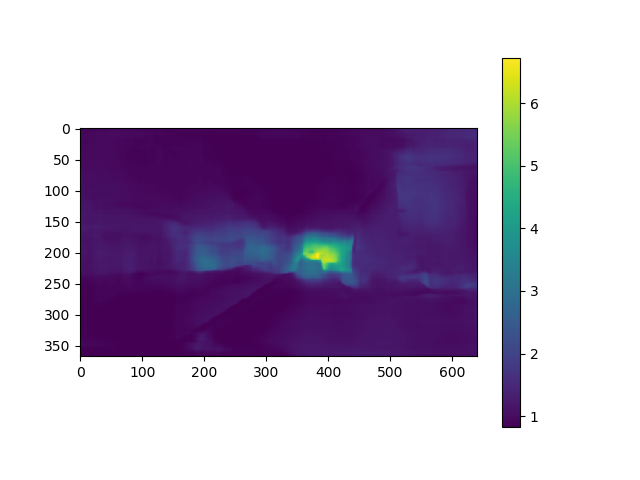
\includegraphics[width=12cm]{figs/preex1.png}
  \end{center}
  \caption{FCRN-DepthPredictionを用いた予備実験}
  \label{fig:preex1}

 \begin{center}
  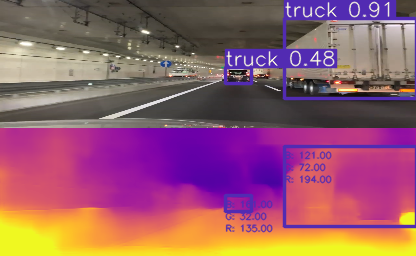
\includegraphics[width=12cm]{figs/preex2.png}
 \end{center}
  \caption{Google Tensorflowを用いた予備実験}
  \label{fig:preex2}
\end{figure}

\newpage
% 動画への適用 ---------------------------------
% 画像処理の話
\section{予備実験2 - 動画への適用}
ここでは2つめに行った予備実験について述べる.
\subsection{実験内容}
この予備実験は,予備実験1にて行ったシステムを動画へ適用する際に行った実験である.
予備実験1では使用した二つのライブラリ(物体検出ライブラリと深度推定ライブラリ)はどちらも画像のデーターを中間ファイルを通して処理していた.
しかし,動画を使った画像処理をこなうためには,中間ファイルを経由しての処理は余分な処理を増やしてしまい,処理量と処理時間がかかってしまう問題がある.
そのため,今後は中間ファイルを経由することなくデータをやり取りするように実行した.
その際に,深度推定ライブラリ(struct2depth)に合わせて画像サイズを416 * 128の高さの半分である 416 * 64サイズに圧縮して処理するよう実装した.
しかし,画像サイズが圧縮されたため,物体検出ライブラリでの誤検出や検出できないといった問題が起きた.

\subsection{症例}
画像を圧縮してから検出を行った際に起きたミスとしては2つあり,それぞれ誤検出と検出できないという症例である.
その検出結果を\figref{fig:miss1}と\figref{fig:miss2}に示す.

% --------------------------------------------------
\newpage
\begin{figure}[htbp]
  \begin{center}
   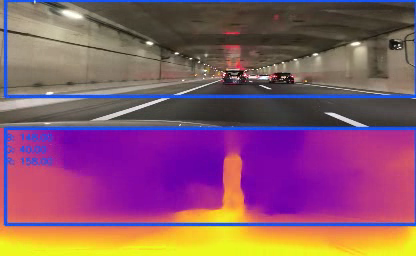
\includegraphics[width=12cm]{figs/miss_1.png}
  \end{center}
  \caption{症例1 - 誤った検出}
  \label{fig:miss1}
\end{figure}

\begin{figure}[hbtp]
 \begin{center}
  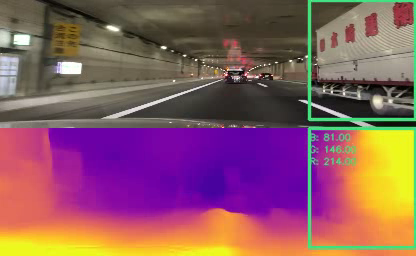
\includegraphics[width=12cm]{figs/miss_2.png}
 \end{center}
  \caption{症例2 - 自動車を検出できなかった症例}
  \label{fig:miss2}
\end{figure}

\newpage
% ---------------------------------------------------

\subsection{解決アプローチ}
症例の原因は元の深度推定ライブラリに合わせて画像を圧縮したため,物体検出システムがうまく機能しなかったためだと考えられる.
問題の解決のため,画像圧縮を避けて画像サイズを416 * 256のまま処理できるように改良した.
その結果,症例で見られるような誤検出や自動車を検出できないといった症例はほとんど見られなくなった.
また,信号機や建物等,渋滞の推定のために必要のない物体を検出しないように,検出物体を自動車類(車,バス,トラック)に絞った.
その実装したプログラムを同じ画像フレームを用いて実験した結果を以下に示す.

% --------------------------------------------------
\begin{figure}[htbp]
  \begin{minipage}{0.5\hsize}
   \begin{center}
    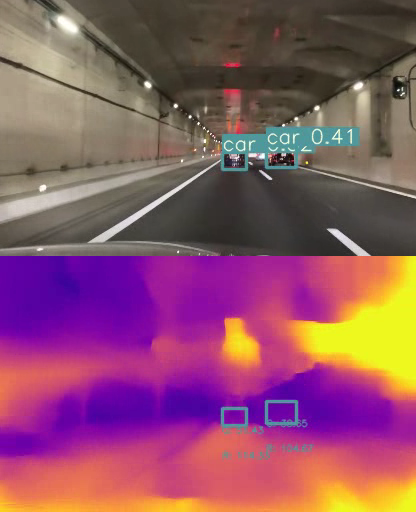
\includegraphics[width=7cm]{figs/pre1_after.png}
   \end{center}
   \caption{症例1の解決}
   \label{fig:pre2after1}
  \end{minipage}
  \begin{minipage}{0.5\hsize}
  \begin{center}
   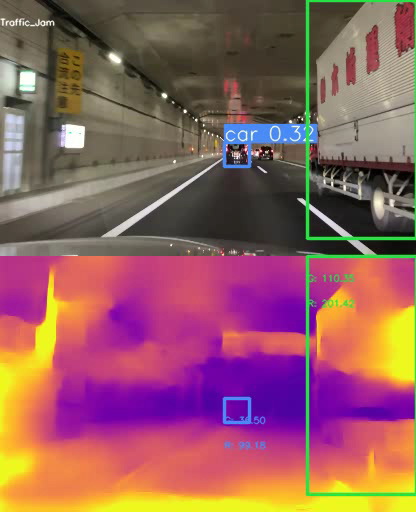
\includegraphics[width=7cm]{figs/pre1_after2.png}
  \end{center}
   \caption{症例2の解決}
   \label{fig:pre2after2}
  \end{minipage}
 \end{figure}

% ---------------------------------------------------
\figref{fig:miss1}と\figref{pre2after1},および\figref{fig:miss2}と\figref{pre2after2}を比較すると,画像の圧縮を抑えた分,誤検出や検出できていない問題が大幅に改善できていることがわかる.
この予備実験2の結果を踏まえて,今後使用する映像圧縮サイズは416 * 256サイズとし,最終的に出力されるサイズはstrct2depthのデーターを加えた416 * 512サイズとする.

\newpage
\section{予備実験3 - 評価方法の決定}
ここでは3つめに行った予備実験について述べる.
\subsection{実験内容}
この予備実験は,本研究における渋滞の評価の基準を決める実験である.
本研究にて使用する深度推定システム(struct2depth)\cite{casser2019struct2depth}は奥行きを推定するシステムだが,\figref{fig:preex2}の通り,結果は色情報でしかわからず,具体的にカメラからどれだけの距離があるのかが不明である.
そのためこの予備実験2では渋滞評価のために出力された色データーから渋滞の基準を決める実験を行う.
本研究では渋滞を車間距離を利用して推定する手法をとっているため,車間距離によって車のスピードや渋滞がどのように変化するかを参考にする.
基本的に車間距離と速度の関係は一般道と高速道路で異なる.
高速道路においては警視庁指示要項によると走行中の車間距離は「速度の2乗/100」をおおよその安全追随距離としている\cite{highway}.
この場合,時速80kmで走っている場合,安全な車間距離は64mとなる.
これに対して高速道路において渋滞している場合の速度は,渋滞の定義を参照すると安全な車間距離は最大で16mとなっている.
しかし,一般道での車間距離は異なる.信号待ち等での停車中の車間距離はトヨタのwebサイトによるとおよそ車一台分,4〜5mとされている\cite{toyota_web}.
よってこの予備実験においては実際に車間距離が4m,5m,6mの時にstruct2depthにおける値がどのように変化するかを調べ,評価基準を決める.


\subsection{使用するデーター}
ここでは予備実験2にて扱うデーターについて述べる.
この予備実験においては実際に車間距離を4m, 5m, 6mのそれぞれにおいて運転席から撮影した映像を利用する.
その際,自動車のフロントガラスにおいて様々な場所から撮影した.以下にサンプルを示す.

% --------------------------------------------------

\begin{figure}[htbp]
  \begin{tabular}{c}
    \begin{minipage}{0.33\hsize}
      \begin{center}
   \includegraphics[width=4.5cm]{figs/sumple/4m_01.png}
    \end{center}
  \caption{車間距離4m}
  \label{fig:sumple4}
\end{minipage}

  \begin{minipage}{0.33\hsize}
  \begin{center}
    \includegraphics[width=4.5cm]{figs/sumple/5m_02.png}
  \end{center}
  \caption{車間距離5m}
  \label{fig:sumple5}
\end{minipage}

  \begin{minipage}{0.33\hsize}
  \begin{center}
    \includegraphics[width=4.5cm]{figs/sumple/6m_01.png}
  \end{center}
  \caption{車間距離6m}
  \label{fig:sumple6}
\end{minipage}
\end{tabular}
\end{figure}

% ---------------------------------------------------
\subsection{実験方法}
ここでは予備実験3で行った実験方法について述べる.
上記の項で示したサンプルデーターをstruct2depth及びYoloシステムを利用して,それぞれの距離においてstrct2depthの数値がどのように変わるかを調べた.
その際,OpenCVの色情報取得システムを利用し,また検出されたBOXの中においてRGB値それぞれの最大値と平均値を比較しどちらを利用すると良いかについても調べた.
その結果の一部を以下に示す.

% ------------------------------------------------------------

\begin{figure}[htbp]
  \begin{tabular}{c}
    \begin{minipage}{0.33\hsize}
      \begin{center}
   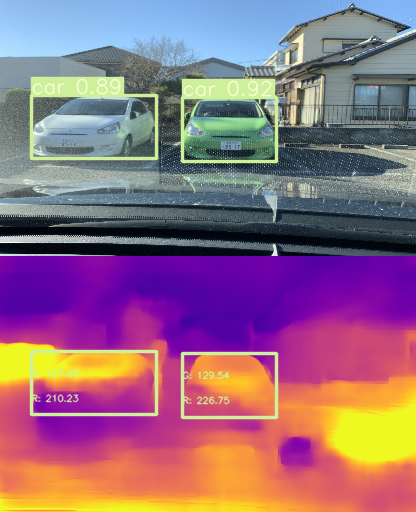
\includegraphics[width=4.5cm]{figs/sumple/4m_02mean.png}
    \end{center}
  \caption{車間距離4m時の平均値}
  \label{fig:sumple4mean}
\end{minipage}

  \begin{minipage}{0.33\hsize}
  \begin{center}
    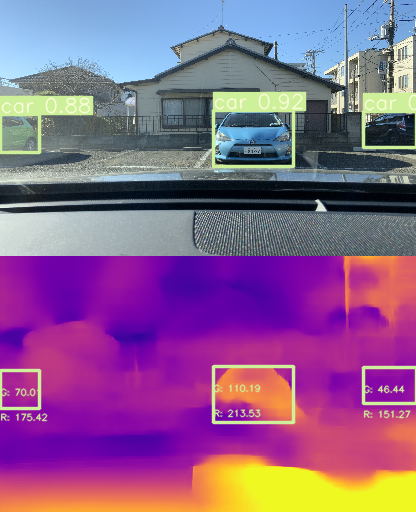
\includegraphics[width=4.5cm]{figs/sumple/5m_02mean.png}
  \end{center}
  \caption{車間距離5m時の平均値}
  \label{fig:sumple5mean}
\end{minipage}

  \begin{minipage}{0.33\hsize}
  \begin{center}
    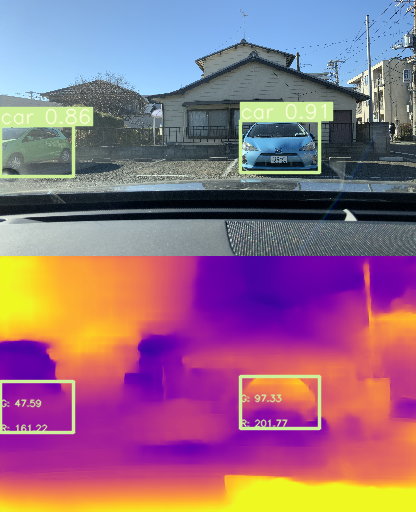
\includegraphics[width=4.5cm]{figs/sumple/6m_01mean.png}
  \end{center}
  \caption{車間距離6m時の平均値}
  \label{fig:sumple6mean}
\end{minipage}
\end{tabular}
\end{figure}

% ------------------------------------------------------------

\begin{figure}[htbp]
  \begin{tabular}{c}
    \begin{minipage}{0.33\hsize}
      \begin{center}
   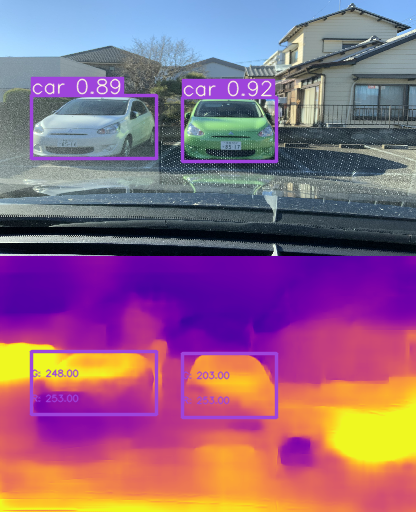
\includegraphics[width=4.5cm]{figs/sumple/4m_02max.png}
    \end{center}
  \caption{車間距離4m時の最大値}
  \label{fig:sumple4max}
\end{minipage}

  \begin{minipage}{0.33\hsize}
  \begin{center}
    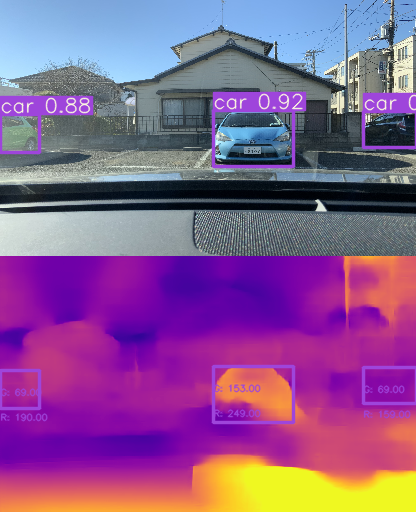
\includegraphics[width=4.5cm]{figs/sumple/5m_02max.png}
  \end{center}
  \caption{車間距離5m時の最大値}
  \label{fig:sumple5max}
\end{minipage}

  \begin{minipage}{0.33\hsize}
  \begin{center}
    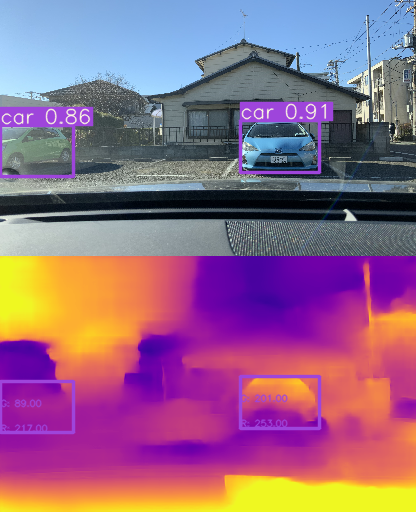
\includegraphics[width=4.5cm]{figs/sumple/6m_01max.png}
  \end{center}
  \caption{車間距離6m時の最大値}
  \label{fig:sumple6max}
\end{minipage}
\end{tabular}
\end{figure}

% ---------------------------------------------------

また,画像の中のR値とG値を改めて以下に表にまとめる.その際,まとめる数値は画面中央に近い自動車の検出された値とする.

% ----------------------------------------------------
\begin{table}[htbp]
  \centering
  \begin{scriptsize}
  \begin{tabular}{ccccccc}
  \toprule
& & 平均値 & 最大値 & & 平均値 & 最大値 \\
  \midrule
4m & R値 & 226.75 & 253.00 & G値 & {\bf129.54} & 203.00 \\
5m & R値 & 213.53 & 249.00 & G値 & {\bf 110.19} & 153.00 \\
6m & R値 & 201.77 & 253.00 & G値 & {\bf 97.33} & 201.00\\
  \bottomrule
  \end{tabular}
  \end{scriptsize}
  \caption{距離別の平均値と最大値}
  \label{tab:mean_max}
\end{table}
% ------------------------------------------------------

\subsection{評価基準の作成}
\tabref{tab:mean_max}からわかることはR値は平均値と最大値のどちらにおいても距離との相関関係は薄いが,G値の特に平均値は距離が近くなるにつれて値が大きくなる傾向があるということである.
この実験結果をもとに,今後の実験においてはG値の平均値を用い,また予備実験3の実験内容の項で述べた通り,車間距離5mを基準とし,G値が100を下回った際に渋滞していると判断する.

\section{まとめ}
本章では,本研究において実装したシステムに関して行なった予備実験について述べた.
予備実験では使用する深度推定ライブラリの決定,画像圧縮問題の解決および評価基準の決定を行った.
次章では本研究における本実験について述べる.
\chapter{実験}
ここでは、本研究の実験が行なった実験について述べる。

\section{データーセット}
ここでは、本実験に用いたデータセットについて述べる。
本実験ではドライブレコーダーの映像を用いる。
そのドライブレコーダーの映像についてはインターネット上の動画投稿サイトYouTubeに投稿されているドライブレコーダーの車載動画を用いる。
その中でも主観的に渋滞していると思われる動画をピックアップし、データーセットとする。

\section{予備実験}
ここでは、本研究が実験を行うにあたってその準備実験の試行として行なった実験について述べる.


%\subsection{データセット}
%この研究ではドライブレコーダーから得られる映像を用いて実験を行う。
%その際、データーセットとしてYouTube等の動画投稿サイトに投稿されたドライブレコーダーの動画を用いる。

\subsection{予備実験}
本研究ではドライブレコーダーから得られる動画を用いて実験、評価を行うが、その予備実験として動画から切り出された画像を用いて本研究のシステムの実験を行った。
この予備実験は、本研究を行うにあたって、距離推定プログラムあるいは深度推定プログラムの候補が2つあり、そのどちらが相応しいかを決める実験である。
その結果を\figref{fig:preex}とに示す。
\figref{fig:preex}のように、このシステムは画像を上下二段に切り分け、上段では入力された映像の高さを半分にした画像、下段はその画像を用いて奥行き推定を行ったものである。
また、上段で自動車とトラックを検出し、下段の同じ位置にBBOXを出力している。
下段のBBOX内に出力されているパラメーターは、下段BOX内のRGB値のそれぞれの値を平均した数値である。

\begin{figure}[htbp]
   \begin{center}
    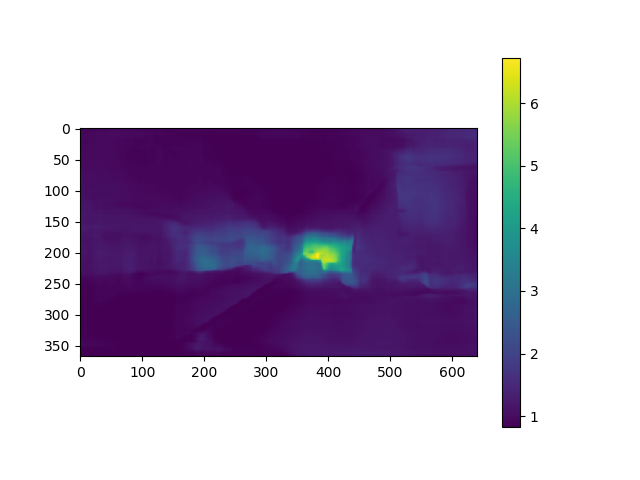
\includegraphics[width=10cm]{figs/preex1.png}
   \end{center}
   \caption{FCRN-DepthPredictionを用いた予備実験}
   \label{fig:preex1}

  \begin{center}
   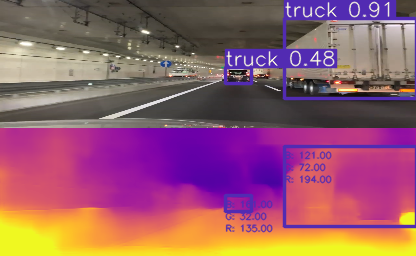
\includegraphics[width=10cm]{figs/preex2.png}
  \end{center}
   \caption{Google Tensorflowを用いた予備実験}
   \label{fig:preex2}
 \end{figure}

\subsection{予備実験 - 評価}
ここでは、本研究における予備実験の評価について述べる。
\figref{fig:preex1}と\figref{fig:preex2}を比較すると、前者は深度推定を行なった結果のみを出力するのに対し、後者は元の画像を圧縮し上下二段二分けて出力されていることがわかる。
また、前者は奥にある物体が明るく色分けされているが、カメラから近いところにある道路やトラックなど、ほぼ暗い青色で塗り分けられているだけであり、物体の識別が難しい。
それに対して後者はカメラから近い距離にある物体ほど明るく塗り分けられており、奥にある物体ほど暗い色になっている。
前者と後者を比較した際、特に違いが顕著なのは後者のシステムの方が画面左側にあるトラックをはっきりと色分けできているという点である。
そのため、本研究においては後者のGoogle Tensorflowを採用し、本実験を行うことにする。

また、\figref{fig:preex2}を見ればわかる通り、物体検出システムと距離推定システムを用いることで先行車との大まかな車間距離を調べることが可能なことがわかる。
\figref{fig:preex2}においてシステムが検出した自動車をそれぞれ右から車1、車2とおくと、下段のRGB値のそれぞれの平均を見てみると、奥にある車1の方が手前にある車2よりもR,Gの値が低く、Bの値が高いことがわかる。
%距離推定システムは奥行きを手前にある物体ほど色を明るく、奥にある(カメラから距離が遠い)物体ほど暗い青色で色分けするので、このシステムで先行車の位置関係が大まかにわかることが確認できる。
この数値の違いを評価することで先行車との距離を推定し、走行スピードを推定し、渋滞しているかどうかを機械に判断させる。
この予備実験を生かして、本実験では動画を用いた渋滞推定を行う。

\section{本実験}
予備実験にて、本研究で使用するシステムを決定した。この項では動画を用いて実際に渋滞を推定する実験について述べる.

\chapter{評価}
ここでは本研究が行った実験における評価について述べる.

\section{考察}
ここでは本研究における評価をもとに考察について述べる。
\section{結論}
% ほぼtanimuさんのパクリ
ここでは本研究における結論について述べる.
本研究ではドライブレコーダー及び深度推定ライブラリ,物体検出ライブラリを用いた渋滞推定システムDepth2Jamについての提案を行った.
深度推定ライブラリを用いることでカメラからの距離を推量することが可能であり,物体検出ライブラリを用いることで推量したい物体を検出することが可能である.
実験では実際にドライブレコーダー映像をもとに本研究を通して開発したシステムを用いて実証実験を行い,渋滞を推定できているか評価を行った.
本提案手法を通じて今まで設置されたものの実際の活用が少なかったドライブレコーダーがより活用されることが期待される.

% footer
\chapter*{謝辞}
本研究を進めるにあたり,ご指導を頂きました慶應義塾大学環境情報学部教授中澤仁博士に深く感謝いたします.
また,慶應義塾大学中澤研究室の諸先輩方には折りに振れ貴重なご助言を頂きました.
特に慶應義塾大学大学院政策・メディア研究科陳寅特任助教,慶應義塾大学大学院政策・メディア研究科大越匡特任講師には本論文を執筆するにあたってご指導頂きました.
ここに深く感謝の意を表します.
そして,慶應義塾大学大学院博士課程 佐々木航氏,慶應義塾大学大学院博士課程 磯川直大氏,慶應義塾大学大学院修士課程 本木悠介氏,慶應義塾大学大学院修士課程 小澤遼氏,慶應義塾大学大学院修士課程 安井慎一郎氏には本研究に対し多くの時間を割いていただきご指導をいただきました.
特に慶應義塾大学大学院博士課程 佐々木航氏は,レインボーシックスシージを通じてさまざまな戦術を披露していただき,とても参考になりました.
また,安井慎一郎氏には卒論執筆に際してアドバイスをいただいたり,激励いただいたり,バーミヤンを奢っていただきました.ここに感謝致します.
小澤遼氏には研究室における作業スペースが隣だったこともあり,TERMや卒論で励ましていただきました.ここに感謝致します.

陰から研究活動を支えて頂いた,松尾さん,遠藤さんに深く感謝申し上げます.
そして,私のメンターである慶應義塾大学大学院修士課程 柿野優衣氏に深く感謝致します.
柿野氏にはWIPの時からお世話になりました.
特にTERMの時期には意見が噛み合わなかったり,発表前日に発表スライドを大幅に変えてしまったりと大変なご迷惑をおかけしました.
そして同じ研究室の先輩方の,慶應義塾大学大学院修士課程 谷村朋樹氏,慶應義塾大学大学院修士課程 川島寛乃氏,慶應義塾大学大学院修士課程 山田佑亮氏に深く感謝致します.

また研究室の同期として,研究活動に切磋琢磨した野田悠加氏,スウィート哲也キース氏,橘直雪氏,マンタタ・タガツォ・ウイリアム氏,助川友里氏,菅原メリッサ紗良氏,鈴木航平氏,山根卓氏に感謝致します.
そして,違う分野ながらもお互いに卒論の執筆について切磋琢磨し,同時に私の精神面を支えてくださった彼女氏に深く感謝致します.
また,私がブレイクダンスをやらなくなってしまってからも,積極的にダーツ等の遊びに誘っていただいた友人の岩間大輝氏に深く感謝致します.

最後に両親へ心から深く感謝を述べます.
前大学での1年半の学費及び生活費を支援してくれたにもかかわらず,中退してしまったことをこの場を借りて改めて謝罪します.
一度中退してしまった私に,半年の海外語学留学と,1年間の北九州予備校での浪人というチャンスをいただき,慶應義塾大学の塾生となることができました.
ここに深く感謝します。

\begin{flushright}
2020年1月21日\\
李 広耀
\end{flushright}


\bibliographystyle{junsrt}
\bibliography{ref.bib}

\appendix
% \def\thesection{付録\Alph{section}}
% \input{append}

\end{document}